\section{Работа с мелодическими контурами}

\subsection{Исходная монотонная запись}

Фраза <<Студент писал реферат>> записана монотонно --- на одном тоне и
без выделения какого-либо слова (файл \texttt{mono\_student.wav}).
Измеренный контур $F_0$ показал медианное значение 124~Гц при разбросе
112--165~Гц: полностью постоянного тона при естественном произнесении
добиться трудно, остаётся небольшой подъём на ударном слоге слова
<<студент>>. Границы слов по осциллограмме: <<студент>> ---
0,99--1,78~с, <<писал>> --- 1,90--2,58~с, <<реферат>> ---
2,78--3,46~с.

\subsection{Методика преобразований}

В программе Sound Forge для работы с мелодическими контурами
используются режимы \texttt{Effect -> Pitch -> Bend} (плавное изменение
$F_0$), \texttt{Effects -> Pitch -> Shift} (постоянный сдвиг тона),
\texttt{Process -> Fade -> Graphic} (изменение амплитуды) и
\texttt{Process -> Time Stretch} (изменение длительности). В данной
работе эти операции реализованы программно:
\begin{itemize}
	\item \emph{Pitch Bend} --- коэффициент изменения тона $r(t)$
	рассчитывается как отношение целевого контура $F_0$ к исходному;
	сигнал обрабатывается блоками по 120~мс с перекрытием 60~мс, внутри
	блока выполняется ресемплинг (тон $\times r$) и фазовый вокодер
	(возврат к исходной длительности); блоки складываются с окном Ханна;
	\item \emph{Pitch Shift} --- та же операция с постоянным $r$ для всего
	сигнала;
	\item \emph{Fade} --- плавное (с фронтами 20~мс) изменение амплитуды
	ударного слова в 1,7 раза при ослаблении остальных в 0,8 раза;
	\item \emph{Time Stretch} --- удлинение ударного слова в 1,35 раза
	фазовым вокодером без изменения тона.
\end{itemize}

Целевые контуры задавались по схеме интонационных типов: для
завершённости --- общее понижение тона от 140 к 110~Гц с локальным
максимумом на ударном слове (смещённым влево), для вопроса --- ровный
тон с максимумом на ударном слове и конечным подъёмом на 75~Гц.

\subsection{Результаты}

Синтезированы шесть вариантов интонации: завершённость и вопрос с
ударением на первое, второе и третье слово. Медианные значения $F_0$
слов и превышение ударного слова над остальными приведены в
таблице~\ref{tab:melody}, контуры --- на рис.~\ref{fig:melody-f0}.

\begin{table}[H]
	\centering
	\small
	\caption{Медианная $F_0$ слов после наклона тона и превышение
		ударного слова над остальными}
	\label{tab:melody}
	\begin{tabular}{|l|l|l|l|l|l|}
		\hline
		Вариант & Слово 1, Гц & Слово 2, Гц & Слово 3, Гц &
		Ударное слово & Превыш., пт \\
		\hline
		исходная & 128 & 126 & 119 & --- & --- \\
		\hline
		заверш., 1-е & \textbf{180} & 123 & 113 & <<Студент>> & $+7{,}2$ \\
		\hline
		заверш., 2-е & 134 & \textbf{154} & 113 & <<писал>> & $+3{,}7$ \\
		\hline
		заверш., 3-е & 134 & 123 & \textbf{152} & <<реферат>> & $+2{,}8$ \\
		\hline
		вопрос, 1-е & \textbf{175} & 130 & 147 & <<Студент>> & $+4{,}1$ \\
		\hline
		вопрос, 2-е & 131 & \textbf{157} & 147 & <<писал>> & $+2{,}1$ \\
		\hline
		вопрос, 3-е & 131 & 131 & \textbf{192} & <<реферат>> & $+6{,}6$ \\
		\hline
	\end{tabular}
\end{table}

\begin{figure}[H]
	\centering
	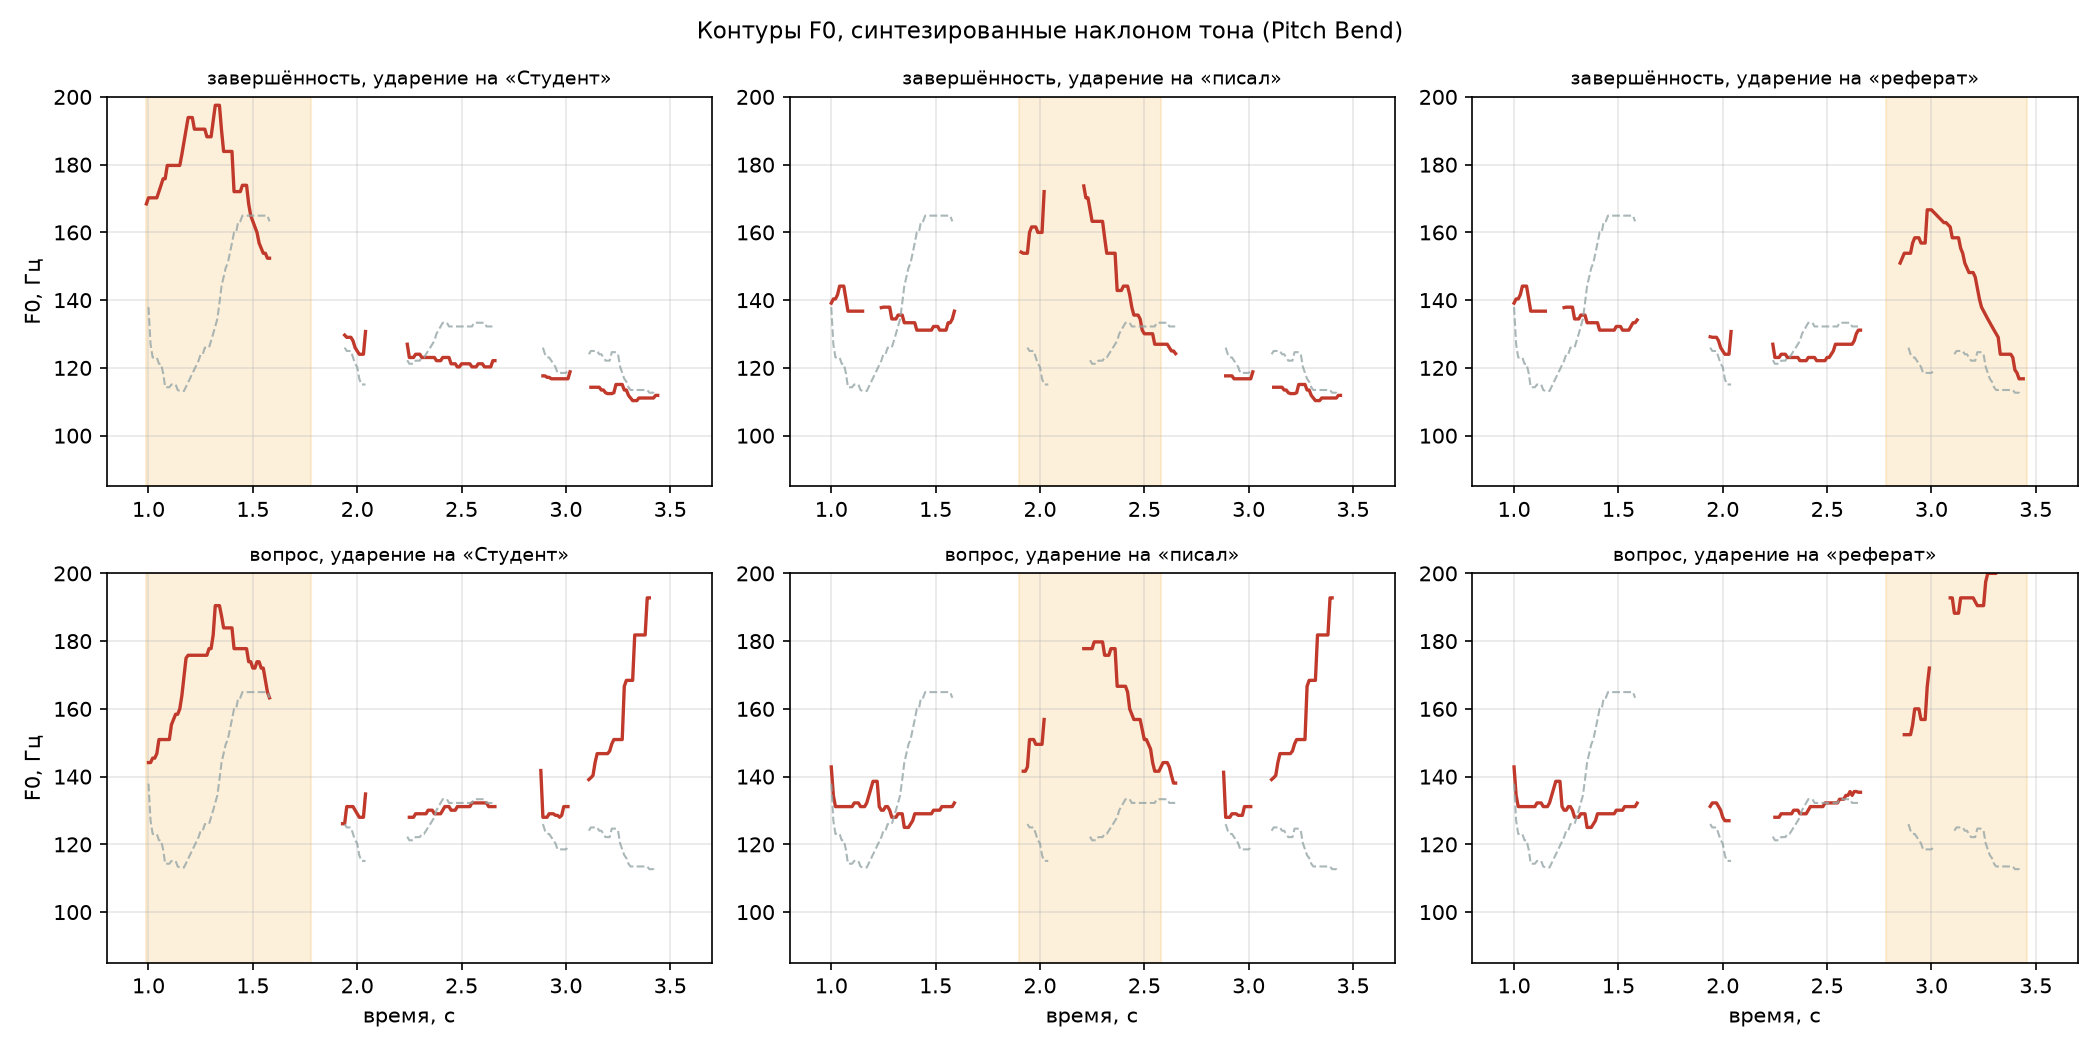
\includegraphics[width=\textwidth]{lab2_melody_f0_contours.png}
	\caption{Контуры $F_0$, синтезированные наклоном тона: интонация
		завершённости (сверху) и вопроса (снизу) с ударением на разные
		слова; штриховой линией показан исходный монотонный контур}
	\label{fig:melody-f0}
\end{figure}

Во всех вариантах ударное слово становится локальным максимумом
мелодического контура: превышение над остальными словами составляет от
2 до 7~полутонов. В вариантах с интонацией вопроса конечный подъём тона
дополнительно повышает $F_0$ последнего слова (до 192~Гц), что
соответствует вопросительной интонации.

Усиление амплитуды ударного слова (\texttt{Fade}) и увеличение его
длительности (\texttt{Time Stretch}) делают фразовое ударение более
отчётливым (рис.~\ref{fig:melody-amp}): уровень ударного слова
возрастает примерно на 5~дБ, а его длительность --- в 1,35 раза.

\begin{figure}[H]
	\centering
	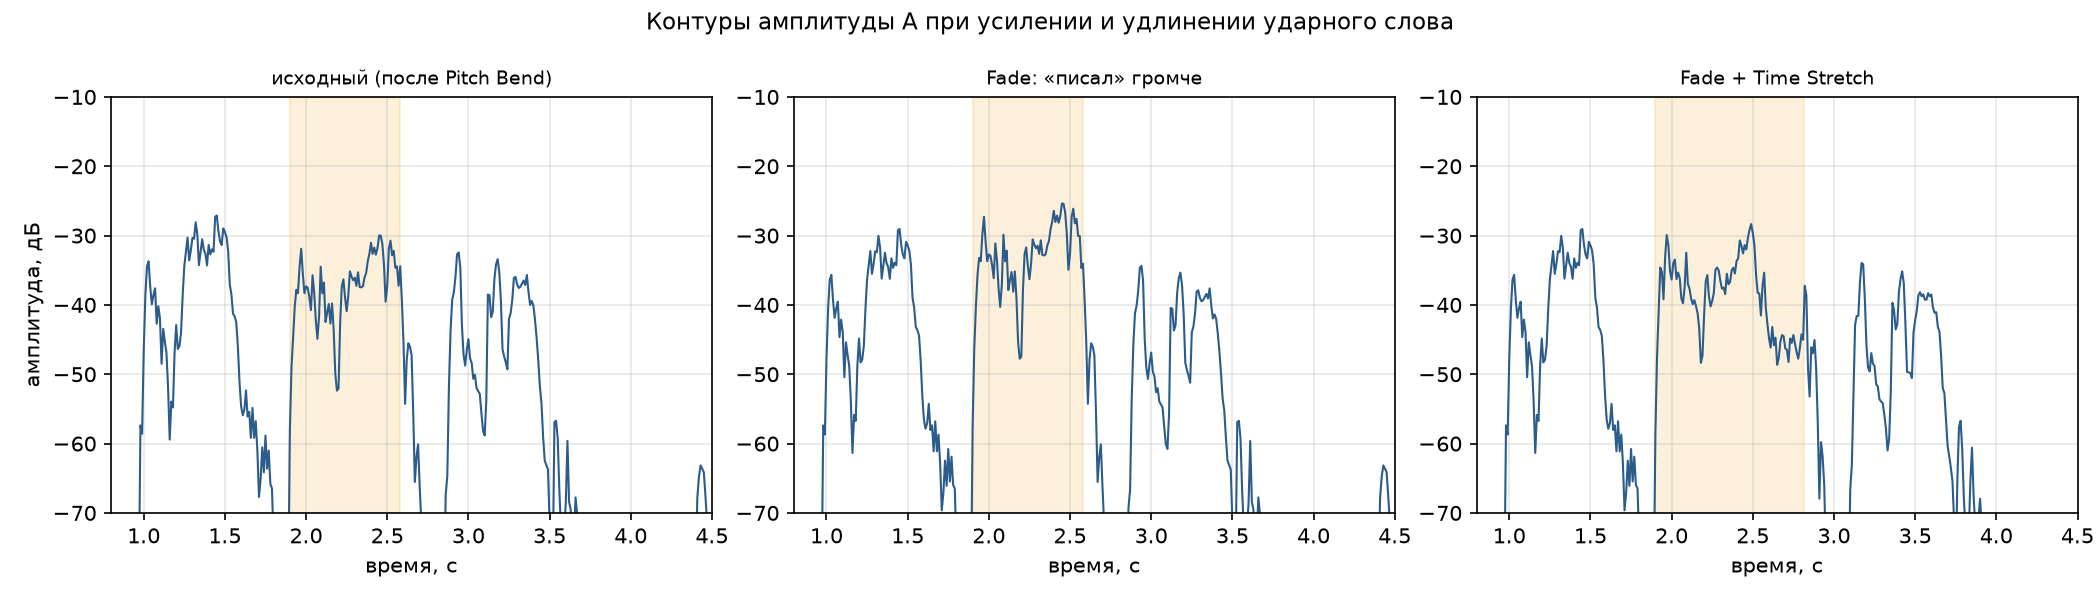
\includegraphics[width=\textwidth]{lab2_melody_amplitude.png}
	\caption{Контуры амплитуды $A$: исходный вариант после наклона тона,
		после усиления ударного слова и после усиления с удлинением}
	\label{fig:melody-amp}
\end{figure}

\subsection{Сравнение Pitch Bend и Pitch Shift}

Для второй копии записи выполнены преобразования режимом Pitch Shift:
постоянный сдвиг тона всего сигнала в 1,15 раза (вверх) и в 0,88 раза
(вниз). В отличие от Pitch Bend, который изменяет $F_0$ по заданному
контуру и формирует интонацию, Pitch Shift сдвигает тон всего сигнала
целиком: мелодический рисунок (соотношение тонов между слогами)
сохраняется, но тембр голоса меняется --- форманты смещаются вместе с
основным тоном. Поэтому для синтеза интонации необходим именно наклон
тона по контуру, а постоянный сдвиг пригоден лишь для изменения высоты
голоса диктора.

Проведённые эксперименты показывают, что фразовое ударение формируется
тремя взаимодополняющими средствами: мелодическим максимумом $F_0$ на
ударном слове, повышением его амплитуды и увеличением длительности.
Совместное применение наклона тона, усиления и растяжения даёт наиболее
отчётливое звучание ударения.
